\documentclass[11pt,a4paper]{article}

\usepackage[margin=2.5cm]{geometry}
\usepackage[T1]{fontenc}
\usepackage{lmodern}
\usepackage{amsmath,amssymb}
\usepackage{booktabs}
\usepackage{array}
\usepackage{graphicx}
\usepackage{caption}
\usepackage{xcolor}
\usepackage{tikz}
\usetikzlibrary{positioning}
\usepackage[hidelinks]{hyperref}

\graphicspath{{figures/}}

\newcommand{\code}[1]{\texttt{#1}}

\title{Cost of the Certified Action Search:\\
Evaluation of Search Optimisations by Depth}
\author{} % add author
\date{27 October 2026}

\begin{document}
\maketitle

\begin{abstract}
This report measures the cost of an exhaustive search for certified action
sequences as a function of depth, and compares implementations of the pacSTL
predicate evaluation it relies on. On ten detection states of a give-way
crossing, a depth-10 search (400~s lookahead, 2.3 million rollouts) takes
77.3~min on one core with the production code. Sharing geometry between
predicates brings this to 47.7~min ($1.62\times$), compiled root finding to
36.6~min ($2.11\times$), and pruning on the turn rule is estimated to reach
27.3~min ($2.83\times$), all with the same certified sequences. Since the tree
grows by about $4.8\times$ per level, this is worth about two thirds of one
level of depth.
\end{abstract}

%======================================================================
\section{The search}
%======================================================================

The masker certifies an action if some action sequence starting with it
satisfies the manoeuvre specification against the obstacle's reachable tube.
This evaluation asks how long an exhaustive search takes for each depth, where
the time goes, and how much the optimisations save without changing the
certified sequences.

\paragraph{Tree.} There are five yaw-rate commands,
$\dot\psi_{\mathrm{cmd}} \in \{-1, -0.5, 0, 0.5, 1\}~^\circ/\mathrm{s}$, each
held for 40~s, so depth $d$ looks $40d$~s ahead and has $5^d$ sequences. The
crossing-side rule (commanded heading offset $\ge 0$) removes sequences before
they are projected. Each remaining edge is one \emph{rollout}: a 40~s
closed-loop simulation of the Mariner hull and autopilot from the parent's
state, after which the new node is evaluated against the reachable set at
that time step.

\paragraph{Specification.} The run uses \code{maneuver\_verified\_LOS\_turn}.
For a trace of $d$ samples (indices $0,\dots,d-1$),
\begin{align}
  \varphi_d \;=\;& \square\,(\mathrm{occupancy\_clear} \ge 0)
  \;\wedge\; \lozenge_{[d-2,\,d-1]}\,(\mathrm{collision\_possible\_LOS} \le 0)
  \label{eq:spec}\\
  \wedge\;& \square\,\big((\mathrm{course\_alteration} \ge 0) \vee
            (\mathrm{range\_closing} \le 0) \vee
            (\mathrm{target\_starboard} \le 0)\big), \nonumber
\end{align}
with $\theta_{\max} = 20^\circ$, $t_{\mathrm{start}} = 480$~s,
$t_h = 300$~s and certification margin $0$. Sample $k$ is the state after
$k+1$ actions, $40(k+1)$~s after detection. The \emph{always} operators cover
the whole trace; the \emph{eventually} window is the last two samples, so it
moves with the leaf and a deeper search may resolve the collision risk later
(Table~\ref{tab:windows}).

\begin{table}[htbp]
\centering
\caption{Sample windows of $\varphi_d$ by depth. Times are seconds after
detection.}
\label{tab:windows}
\small
\begin{tabular}{@{}rrccc@{}}
\toprule
 & & $\square$ (occupancy, turn rule) & \multicolumn{2}{c}{$\lozenge$ (collision risk resolved)} \\
\cmidrule(lr){3-3}\cmidrule(l){4-5}
$d$ & Lookahead (s) & samples & samples & times (s) \\
\midrule
1 & 40 & $0$ & $\{0\}$ & 40 \\
2 & 80 & $0,\dots,1$ & $[0,1]$ & 40, 80 \\
3 & 120 & $0,\dots,2$ & $[1,2]$ & 80, 120 \\
4 & 160 & $0,\dots,3$ & $[2,3]$ & 120, 160 \\
5 & 200 & $0,\dots,4$ & $[3,4]$ & 160, 200 \\
6 & 240 & $0,\dots,5$ & $[4,5]$ & 200, 240 \\
7 & 280 & $0,\dots,6$ & $[5,6]$ & 240, 280 \\
8 & 320 & $0,\dots,7$ & $[6,7]$ & 280, 320 \\
9 & 360 & $0,\dots,8$ & $[7,8]$ & 320, 360 \\
10 & 400 & $0,\dots,9$ & $[8,9]$ & 360, 400 \\
\bottomrule
\end{tabular}
\end{table}

\paragraph{Incremental evaluation.} A predicate sample depends only on the ego
state and the reachable set at its own time step, not on the rest of the trace
or on the window. Each node therefore computes one new sample and reuses its
ancestors' (Figure~\ref{fig:tree}), and the formula is evaluated once per leaf
over the leaf's trace. Compared with recomputing the whole trace at every
leaf, this needs about eight times fewer predicate samples at depth 10, with
identical values.

\begin{figure}[htbp]
\centering
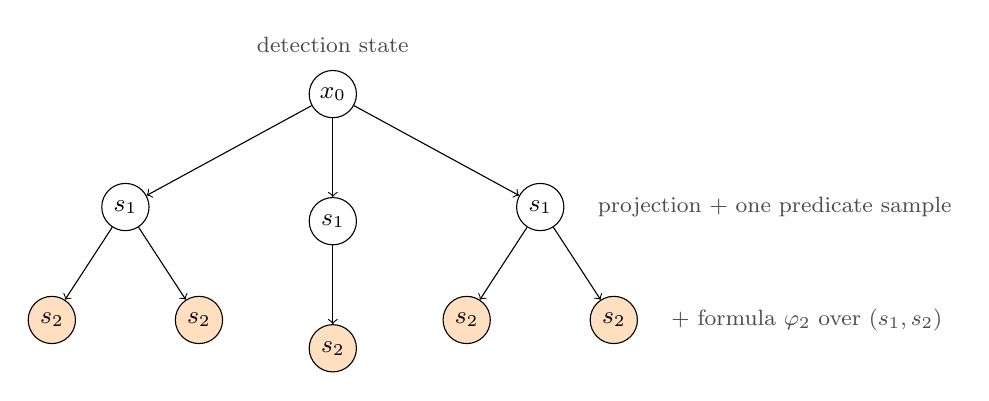
\begin{tikzpicture}[
  node distance=1.0cm and 1.4cm,
  nd/.style={circle,draw,minimum size=6mm,inner sep=0pt,font=\small},
  lf/.style={nd,fill=orange!25},
  lbl/.style={font=\footnotesize,text=black!70}]
  \node[nd] (r) {$x_0$};
  \node[nd,below left=1.0cm and 2.2cm of r] (a) {$s_1$};
  \node[nd,below=1.0cm of r] (b) {$s_1$};
  \node[nd,below right=1.0cm and 2.2cm of r] (c) {$s_1$};
  \node[lf,below left=1.0cm and 0.5cm of a] (a1) {$s_2$};
  \node[lf,below right=1.0cm and 0.5cm of a] (a2) {$s_2$};
  \node[lf,below=1.0cm of b] (b1) {$s_2$};
  \node[lf,below left=1.0cm and 0.5cm of c] (c1) {$s_2$};
  \node[lf,below right=1.0cm and 0.5cm of c] (c2) {$s_2$};
  \foreach \p/\q in {r/a,r/b,r/c,a/a1,a/a2,b/b1,c/c1,c/c2} \draw[->] (\p) -- (\q);
  \node[lbl,right=0.3cm of c] {projection + one predicate sample};
  \node[lbl,right=0.3cm of c2] {+ formula $\varphi_2$ over $(s_1,s_2)$};
  \node[lbl,above=0.1cm of r] {detection state};
\end{tikzpicture}
\caption{Incremental evaluation of a depth-2 tree. Every node projects the
ego for one action and computes one predicate sample; its children reuse it.
The formula is evaluated only at the leaves (shaded). Branches removed by the
crossing-side rule are not drawn.}
\label{fig:tree}
\end{figure}

%======================================================================
\section{Setup}
%======================================================================

The evaluation runs the environment of
\begin{center}
\footnotesize\code{mariner\_40s\_depth4\_turn20stbd\_ts480\_det300\_clean\_det400\_pre\_b02x20\_t2400\_200k}
\end{center}
and stops at the \emph{detection state} (detection horizon 300~s), where the
masker's first and largest search starts. Ten states (reset seeds from 0) are
used for every method; the obstacle is 6.3--10.5~km away at 4.7--7.7~m/s.
The reachable tube (\code{mariner\_40\_b02\_20sets}, one PAC ellipsoid per
40~s) is loaded before the search and not timed. There is no ego uncertainty.
All runs use one node with 40 worker processes.

\paragraph{Time accounting.} The tree to depth 10 is searched once per state
and method, and each node's time is added to its depth. The time of an
exhaustive depth-$d$ search is
\begin{equation}
  T(d) \;=\; \sum_{k=1}^{d} t_{\mathrm{node}}(k) \;-\; \sum_{k=1}^{d-1} t_{\varphi}(k),
  \label{eq:time}
\end{equation}
where $t_{\mathrm{node}}(k)$ is the total time of the depth-$k$ nodes and
$t_{\varphi}(k)$ their formula time. The run evaluates the formula at
every node to count certified sequences per depth, but a depth-$d$ search
needs it only at its leaves, so the second sum removes it. The inner nodes'
projection and predicates stay in, since the leaves need them. All times are
one-core times (summed over processes), median over the ten states.

%======================================================================
\section{Methods}
\label{sec:methods}
%======================================================================

The methods differ only in how a node's predicates are computed (and pruning
in which nodes are visited). They are implemented as variants that replace
production functions at run time (\code{gym/eval/search/variants/}).

\begin{table}[htbp]
\centering
\caption{Methods compared.}
\label{tab:methods}
\small
\begin{tabular}{@{}>{\raggedright\arraybackslash}p{3.1cm}>{\raggedright\arraybackslash}p{8.3cm}>{\raggedright\arraybackslash}p{2.6cm}@{}}
\toprule
Method & Change & Same certificates \\
\midrule
Production & Secular equation solved with \code{scipy.optimize.brentq};
  closed-form linear bounds; incremental trace & reference \\
Shared geometry & Each distinct min/max problem solved once per sample and
  shared by all predicates & yes, bit-identical \\
Compiled roots & Secular equations solved in compiled code (numba) & yes \\
Pruning (estimate) & Sequences dropped once the turn rule has failed & yes, by construction \\
Legacy optimiser & SLSQP over the full 6-D ellipsoid (before 26 Sep 2026) & no \\
Legacy full trace & Every sample of the sequence recomputed at every node & yes \\
\bottomrule
\end{tabular}
\end{table}

\paragraph{Production.} Most predicate bounds are the minimum or maximum of a
squared distance or relative speed over the reachable set projected onto two
dimensions, $\{x : (x-c)^{\top}\Sigma^{-1}(x-c) \le 1\}$ with
$\Sigma = U\Lambda U^{\top}$. For the minimum distance to a point $x_o$, with
$\delta = U^{\top}(x_o - c)$,
\begin{equation}
  \min \lVert x - x_o\rVert^2 = \sum_i \left(\frac{\mu\,\delta_i}{\lambda_i+\mu}\right)^{2},
  \qquad
  \text{where } \mu > 0 \text{ solves } \;
  \sum_i \frac{\lambda_i\,\delta_i^2}{(\lambda_i+\mu)^2} = 1 ,
  \label{eq:secular-min}
\end{equation}
(or $0$ if $x_o$ is inside); the maximum has the same form. The root is found
with \code{brentq} on a Python function, about ten interpreter calls per root.
Linear bounds are closed form, and the per-set geometry is cached. Each
predicate solves its own problems.

\paragraph{Shared geometry.} The turn specification asks for the same minimum
and maximum ego--obstacle distance in four predicates (8 solves for 2 distinct
problems), and two predicates need the same closing-rate bounds. The variant
memoises these per sample, so each distinct problem is solved once. Solver and
inputs are unchanged, so results are bit-identical.

\paragraph{Compiled roots.} The secular equations are solved in numba with
Newton's method on $F(x)^{-1/2} - 1$, which is nearly linear near the poles,
with a bisection fallback and production's tolerances. Results are not
bit-identical but agree within tolerance (Section~\ref{sec:verification}).
It is measured on top of shared geometry.

\paragraph{Pruning (estimate).} The turn rule is an \emph{always}: once its
lower bound at one sample is below the margin, no extension can be certified,
so a search could stop expanding that node. Pruning was not run; the time is
scaled by the share of rollouts that lie below such nodes. No certified
sequence passes through such a node, which confirms the check.

\paragraph{Legacy.} Before 26 September 2026, minimum distance, minimum
relative speed and linear bounds were solved with SLSQP over the full 6-D
ellipsoid. SLSQP is local, so it can return too large a minimum, i.e.\ too
high a lower bound. Also, every node re-evaluated the whole trajectory instead
of reusing its parent's samples (\emph{full trace}). The newer predicates run
on top of both.

%======================================================================
\section{Verification}
\label{sec:verification}
%======================================================================

The per-depth counts (rollouts, certified and extendable sequences) are
identical, state by state, for production, shared geometry and shared
geometry with compiled roots. The legacy optimiser certifies 10 more
sequences at depth 7, in 2 of the 10 states. In addition,
\code{variant\_check} evaluates a random sample of predicate inputs from the
production search with production and with each variant
(Table~\ref{tab:check}). A raised lower bound is unsafe: it can certify a
sequence production does not.

\begin{table}[htbp]
\centering
\caption{Accuracy against production on identical predicate inputs.
``Differing'': relative difference above $10^{-6}$. Predicate-only time per
sample.}
\label{tab:check}
\footnotesize
\setlength{\tabcolsep}{4pt}
\begin{tabular}{@{}lrrrrrr@{}}
\toprule
Method & Samples & Differing & Lower raised & Upper lowered
  & \multicolumn{2}{c}{$\mu$s per sample} \\
\cmidrule(l){6-7}
 & & & & & production & method \\
\midrule
Shared geometry & 198\,473 & 0 & 0 & 0 & 683 & 329 \\
Shared geom.\ + compiled roots & 198\,473 & 0 & 0 & 0 & 683 & 145 \\
Legacy optimiser (plan inputs) & 20\,000 & 2\,199 & 308 & 366 & 673 & 83\,325 \\
Legacy optimiser (turn inputs) & 1\,444 & 1\,734 & 1\,324 & 1\,028 & 650 & 105\,205 \\
\bottomrule
\end{tabular}
\end{table}

The legacy optimiser raises lower bounds in hundreds of samples, in occupancy
by up to $4.8\times10^{3}$ and in course alteration by up to $2.8$.

%======================================================================
\section{Results}
%======================================================================

\subsection{Search time by depth}

\begin{figure}[htbp]
\centering
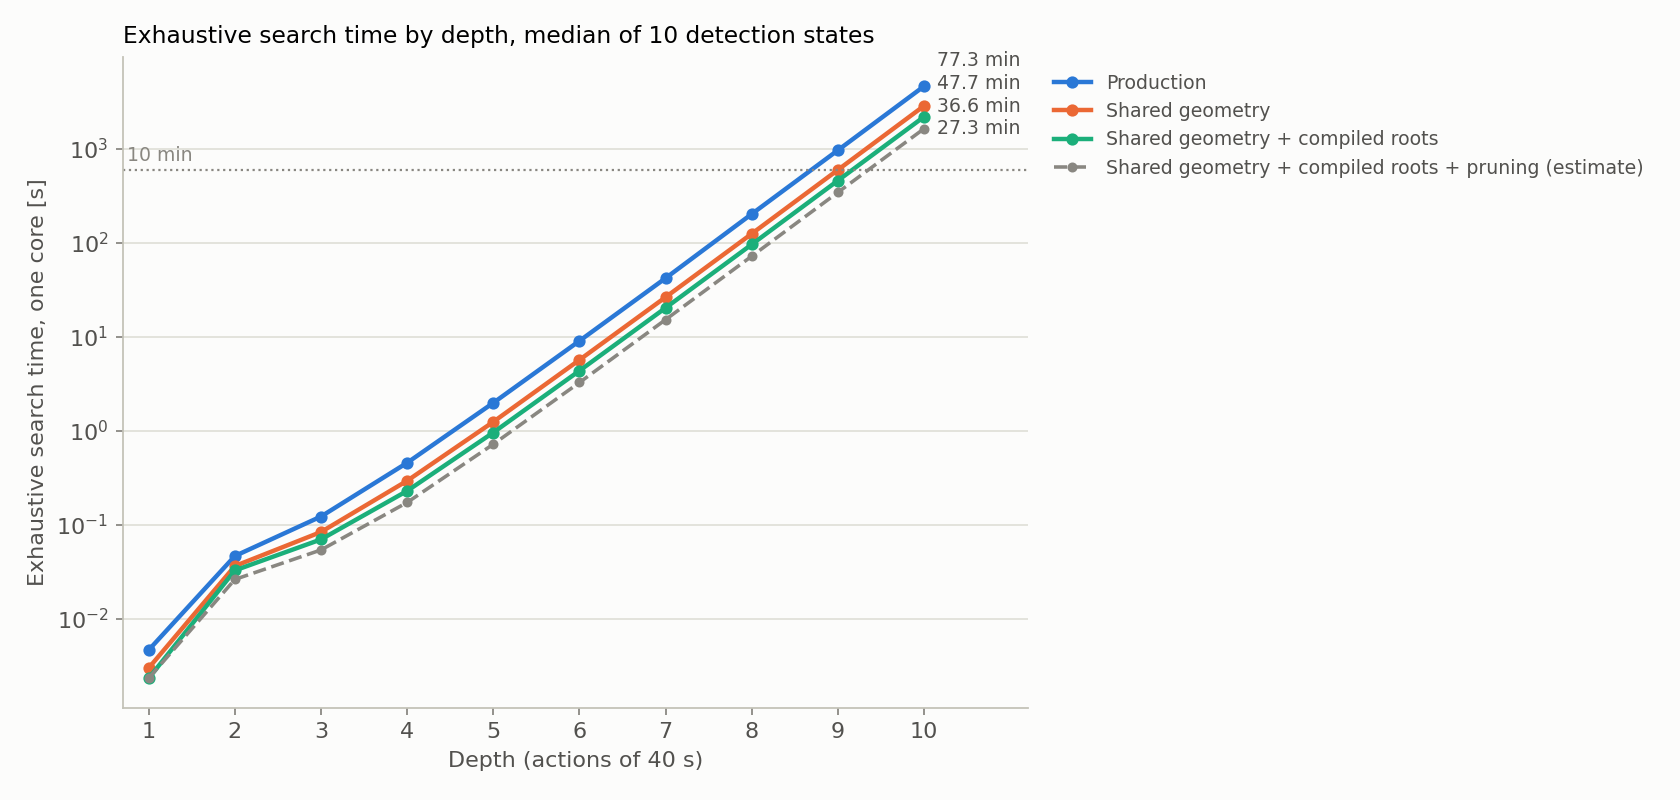
\includegraphics[width=\linewidth]{search_time_by_depth.png}
\caption{One-core time of an exhaustive search by depth, median of 10
detection states (Eq.~\ref{eq:time}). Log scale; the dotted line marks
10~min.}
\label{fig:time}
\end{figure}

\begin{table}[htbp]
\centering
\caption{One-core exhaustive search time by depth (median over 10 states) and
speed-up against production. Each column includes the changes to its left.}
\label{tab:time}
\small
\begin{tabular}{@{}rrrrr@{}}
\toprule
Depth & Production & + shared geometry & + compiled roots & + pruning (est.) \\
\midrule
1  & 0.005 s  & 0.003 s ($1.56\times$) & 0.002 s ($2.00\times$) & 0.002 s ($2.00\times$) \\
2  & 0.05 s   & 0.04 s ($1.28\times$)  & 0.03 s ($1.42\times$)  & 0.03 s ($1.77\times$) \\
3  & 0.12 s   & 0.08 s ($1.46\times$)  & 0.07 s ($1.75\times$)  & 0.05 s ($2.27\times$) \\
4  & 0.46 s   & 0.29 s ($1.55\times$)  & 0.23 s ($1.99\times$)  & 0.17 s ($2.64\times$) \\
5  & 2.0 s    & 1.2 s ($1.59\times$)   & 0.96 s ($2.07\times$)  & 0.72 s ($2.75\times$) \\
6  & 9.0 s    & 5.7 s ($1.59\times$)   & 4.3 s ($2.08\times$)   & 3 s ($2.77\times$) \\
7  & 42 s     & 26 s ($1.59\times$)    & 20 s ($2.07\times$)    & 15 s ($2.76\times$) \\
8  & 3.4 min  & 2.1 min ($1.62\times$) & 96 s ($2.11\times$)    & 72 s ($2.81\times$) \\
9  & 16.1 min & 9.9 min ($1.62\times$) & 7.7 min ($2.10\times$) & 5.7 min ($2.81\times$) \\
10 & 77.3 min & 47.7 min ($1.62\times$)& 36.6 min ($2.11\times$)& 27.3 min ($2.83\times$) \\
\bottomrule
\end{tabular}
\end{table}

From depth 5 on, time grows by $4.5$--$4.8\times$ per level, close to the
growth in nodes, and the speed-ups are nearly constant. At depth 10 the
individual contributions are $1.62\times$ (shared geometry), $1.30\times$
(compiled roots, on top) and $1.34\times$ (pruning, on top). Compiled roots
alone would likely save more, since production solves about four times as
many root problems. The states differ little (75.0--79.0~min at depth 10).

\subsection{Cost per node}

\begin{figure}[htbp]
\centering
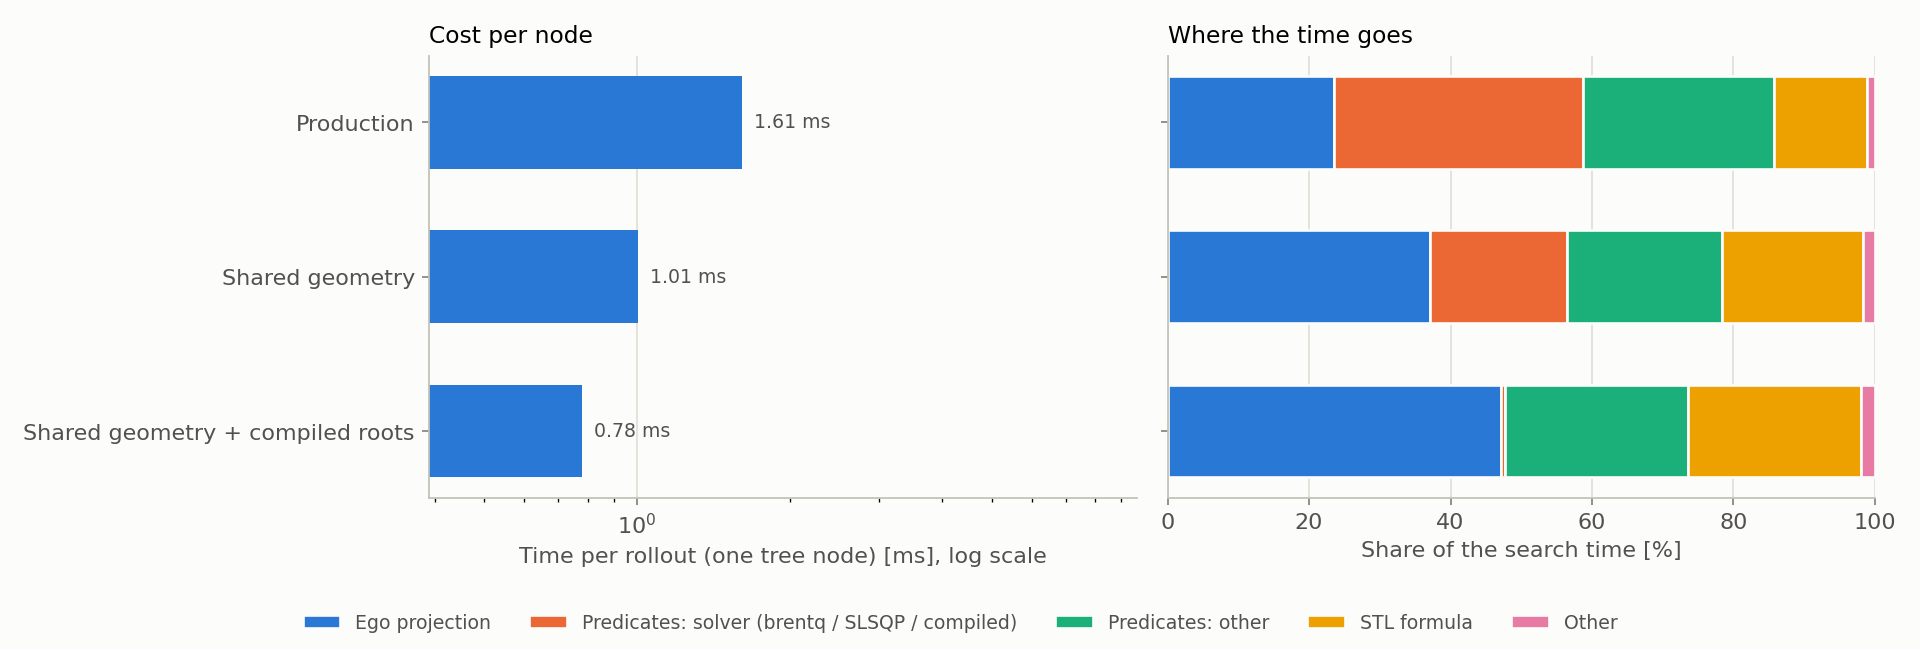
\includegraphics[width=\linewidth]{time_breakdown.png}
\caption{Time per rollout by part, over all depths to 10. The formula is
counted at the depth-10 leaves only and spread over all nodes.}
\label{fig:breakdown}
\end{figure}

\begin{table}[htbp]
\centering
\caption{Time per rollout by part, as in Figure~\ref{fig:breakdown}.}
\label{tab:breakdown}
\small
\begin{tabular}{@{}lrrr@{}}
\toprule
Part & Production & Shared geometry & + compiled roots \\
\midrule
Ego projection & 0.379 ms (24\%) & 0.373 ms (39\%) & 0.367 ms (50\%) \\
Predicates: root finding & 0.567 ms (36\%) & 0.196 ms (20\%) & 0.004 ms (1\%) \\
Predicates: other & 0.434 ms (28\%) & 0.219 ms (23\%) & 0.201 ms (27\%) \\
STL formula & 0.168 ms (11\%) & 0.160 ms (17\%) & 0.152 ms (21\%) \\
Other & 0.018 ms (1\%) & 0.016 ms (2\%) & 0.015 ms (2\%) \\
\midrule
Total & 1.565 ms & 0.965 ms & 0.740 ms \\
\bottomrule
\end{tabular}
\end{table}

In production the predicates take 64\% of the node time. Shared geometry cuts
root finding by about two thirds and other predicate work by half; compiled
roots make root finding negligible. Per sample the predicates become
$4.7\times$ faster (Table~\ref{tab:check}), but per node only $2.1\times$,
because the projection and formula are untouched: even free predicates would
leave 0.56~ms per node, at most $2.8\times$. After both optimisations, the
projection is 50\% of the node time.

\subsection{Legacy implementations}

\begin{figure}[htbp]
\centering
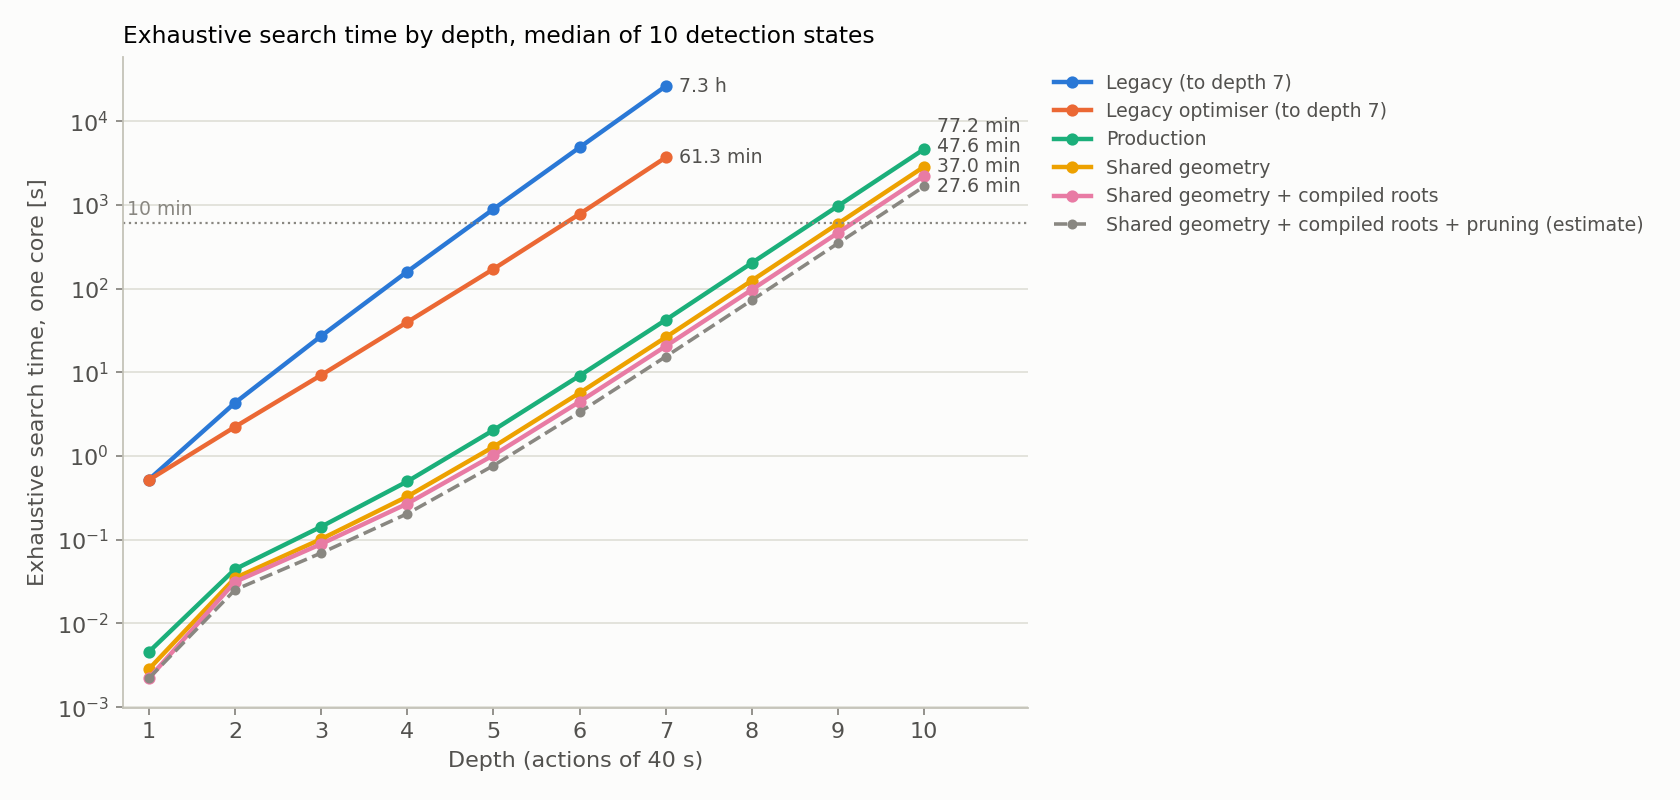
\includegraphics[width=\linewidth]{search_time_legacy.png}
\caption{Search time by depth of production and the legacy implementations,
to depth 7, accounted as in Figure~\ref{fig:time}.}
\label{fig:legacy}
\end{figure}

\begin{table}[htbp]
\centering
\caption{Median one-core search time, production against the legacy
implementations (slow-down relative to production).}
\label{tab:legacy}
\small
\begin{tabular}{@{}rlll@{}}
\toprule
$d$ & Production & Legacy optimiser & Legacy (optimiser + full trace) \\
\midrule
3 & 0.12 s & 9.5 s ($77\times$) & 28 s ($225\times$) \\
4 & 0.46 s & 41 s ($88\times$) & 2.7 min ($353\times$) \\
5 & 2.0 s & 2.9 min ($88\times$) & 15.1 min ($454\times$) \\
6 & 9.1 s & 13.2 min ($87\times$) & 82.7 min ($543\times$) \\
7 & 42 s & 62.3 min ($88\times$) & 7.5 h ($635\times$) \\
\bottomrule
\end{tabular}
\end{table}

At depth 7, the legacy optimiser is $88\times$ slower than production
(132~ms against 1.5~ms per node, almost all in SLSQP), and the full legacy
search $635\times$. Recomputing the whole trace costs $4.0\times$ at depth 4
and $7.2\times$ at depth 7, growing with depth since a depth-$d$ node
recomputes $d$ samples instead of one.

\subsection{Tree size and certified sequences}
\label{sec:tree}

\begin{figure}[htbp]
\centering
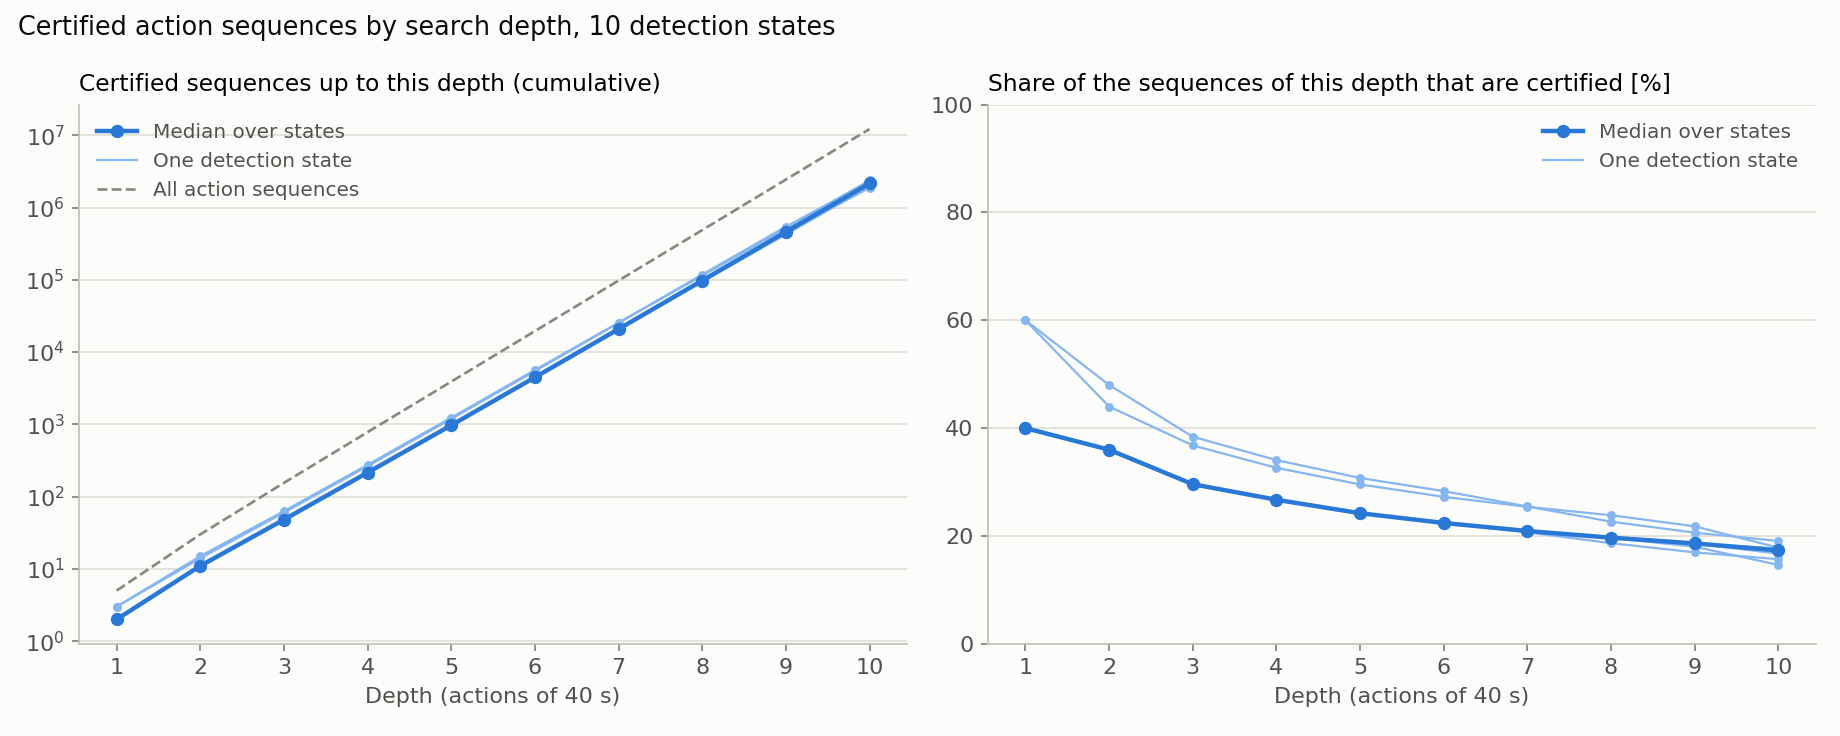
\includegraphics[width=\linewidth]{certified_sequences.png}
\caption{Certified sequences by depth (production). Left: cumulative count,
with all $5^d$ sequences for reference. Right: certified share per depth.}
\label{fig:certified}
\end{figure}

\begin{table}[htbp]
\centering
\caption{Sequences by depth (production, median over states). ``Projected'':
sequences allowed by the crossing-side rule, one rollout each.}
\label{tab:certified}
\small
\begin{tabular}{@{}rrrrr@{}}
\toprule
Depth & All ($5^d$) & Projected & Certified & Certified share \\
\midrule
1  & 5         & 3         & 2         & 40.0\% \\
2  & 25        & 12        & 9         & 36.0\% \\
3  & 125       & 51        & 37        & 29.6\% \\
4  & 625       & 226       & 167       & 26.7\% \\
5  & 3\,125    & 1\,025    & 757       & 24.2\% \\
6  & 15\,625   & 4\,724    & 3\,503    & 22.4\% \\
7  & 78\,125   & 22\,022   & 16\,350   & 20.9\% \\
8  & 390\,625  & 103\,550  & 76\,902   & 19.7\% \\
9  & 1\,953\,125 & 490\,191 & 363\,901 & 18.6\% \\
10 & 9\,765\,625 & 2\,333\,057 & 1\,692\,075 & 17.3\% \\
\bottomrule
\end{tabular}
\end{table}

The crossing-side rule removes about three quarters of the sequences, mostly
in the first levels where only 3 of 5 actions are allowed; from depth 5 on,
the projected sequences grow by about $4.8\times$ per level. With the
obstacle 6--10~km away, no node breaks the safety radius, so the tree has the
same 2\,954\,861 nodes in every state and no predicate solve is wasted on a
dead branch. The certified share falls from 40\% to 17\% with depth, and about
25\% of the rollouts lie below a failed turn rule, which is what pruning would
save.

%======================================================================
\section{Discussion and conclusion}
%======================================================================

A depth-10 exhaustive search costs 77~min on one core in production. Shared
geometry and compiled roots reduce this to 37~min ($2.11\times$) with the same
certified sequences, and pruning on the turn rule is estimated to reach 27~min
($2.83\times$). The legacy SLSQP optimiser was $88\times$ slower than
production and could raise lower bounds, which is unsafe for certification.

Because the tree grows by about $4.8\times$ per level, a speed-up $s$ is worth
$\ln s/\ln 4.8$ levels: $2.83\times$ is about $0.66$ of a level (26~s of
lookahead). With a 10-minute one-core budget, production reaches depth 8 and
the optimised search with pruning depth 9; depth 10 remains out of reach, so
deeper certificates need fewer branching levels (for example longer holds at
later levels), not only faster nodes. After the optimisations, the ego
projection is half the node time; pruning is the cheapest remaining gain, and
incremental formula monitoring and parallel subtrees are further options.

\paragraph{Limitations.} The exhaustive tree is the cost of the phased plan;
the receding mask stops at the first certified leaf per first action, so these
times are an upper bound for it. Only the detection state of one crossing was
evaluated; later states have smaller trees. The pruning result is an estimate
assuming a pruned rollout costs as much as an average one. Each state and
method was run once; the ten states agree within $\pm 3\%$.

\appendix
%======================================================================
\section{Reproduction}
%======================================================================

From \code{colregs\_gym/}, \code{jobs/eval/search\_compare\_turn\_d10.slurm}
runs, for each method,
\begin{verbatim}
python -m gym.eval.search.search_tree configuration/<run>.yaml \
    --depth 10 -n 10 --seed 0 --split 2 --profile-parts \
    --variant <baseline|shared_geometry|numba_roots+shared_geometry> \
    --workers 40
\end{verbatim}
{\sloppy and then \code{python -m gym.eval.search.compare}. The legacy
comparison (\code{search\_compare\_legacy\_d7.slurm}) does the same at depth 7
with \code{legacy\_optimizer} and \code{legacy\_optimizer+legacy\_full\_trace}.
The accuracy check is \code{python -m gym.eval.search.variant\_check}. Code is
in \code{gym/eval/search/} (variants in \code{variants/}), results in
\code{gym/eval/search/results/<config>/}.\par}

\end{document}
